\documentclass[a4paper,14pt]{report}
\usepackage[T2A]{fontenc}
\usepackage[utf8]{inputenc}
\usepackage[english,russian]{babel}
\usepackage{listings}
\usepackage{geometry}
\usepackage{amssymb}
\usepackage{amsmath}
\usepackage[14pt]{extsizes}
\geometry{left=2cm}
\geometry{right=1.5cm}
\geometry{top=1cm}
\geometry{bottom=2cm}
\pagestyle{plain}
\usepackage{pgfplots}
\usepackage{filecontents}
\usepackage{graphicx}
\usepackage{indentfirst}
\DeclareGraphicsExtensions{.png}
\graphicspath{{images/}}
\usetikzlibrary{datavisualization}
\usetikzlibrary{datavisualization.formats.functions}
\usepackage{tabularx}
\pgfplotsset{width=7 cm}

\usepackage{tocloft}

\renewcommand\cftchapdotsep{\cftdot}
\renewcommand\cftsecdotsep{\cftdot}
\renewcommand{\cftchapleader}{\cftdotfill{\cftchapdotsep}}

%Четные
%Размер массива	0, 1, ... 16
%100 & 38 & 16 & 9 & 10 & 8 & 9 & 8 & 8 & 7 & 8 & 8 & 8 & 7 & 8 & 8 & 8 & 8 &
%200 & 133 & 133 & 66 & 80 & 62 & 66 & 66 & 63 & 63 & 63 & 62 & 63 & 62 & 62 & 62 & 63 & 61 &
%300 & 457 & 452 & 228 & 242 & 210 & 215 & 218 & 218 & 216 & 214 & 213 & 214 & 213 & 212 & 212 & 210 & 212 &
%400 & 1080 & 1077 & 541 & 539 & 501 & 523 & 515 & 516 & 510 & 506 & 503 & 508 & 505 & 504 & 506 & 505 & 506 &
%500 & 2147 & 2155 & 1073 & 1089 & 998 & 1032 & 1002 & 1006 & 995 & 1001 & 1009 & 1007 & 1098 & 1211 & 987 & 985 & 986 &
%600 & 3861 & 3728 & 2019 & 1817 & 1710 & 1766 & 1762 & 1827 & 1716 & 1734 & 1719 & 1717 & 1746 & 1826 & 1717 & 1714 & 1714 &
%700 & 6115 & 6063 & 3042 & 2973 & 2855 & 2776 & 2792 & 2768 & 2871 & 2777 & 2749 & 2746 & 2867 & 2769 & 2753 & 2749 & 2745 &
%800 & 9408 & 9288 & 4625 & 4634 & 4191 & 4306 & 4388 & 4214 & 4210 & 4340 & 4229 & 4215 & 4306 & 4230 & 4210 & 4321 & 4207 &
%900 & 13870 & 13724 & 7087 & 6639 & 6330 & 6253 & 6358 & 6242 & 6320 & 6254 & 6355 & 6211 & 6340 & 6246 & 6370 & 6199 & 6341 &
%1000 & 19275 & 19374 & 10407 & 9806 & 9089 & 9324 & 9310 & 9214 & 9181 & 9284 & 9259 & 9161 & 9196 & 9264 & 9321 & 9115 & 9238 &

\begin{filecontents}{noThreadEven.dat}
	100 16
	 200 133
	 300 452
	 400 1077
	 500 2147
	 600 3728
	 700 6063
	 800 9288
	 900 13724
	 1000 19275
\end{filecontents}

\begin{filecontents}{thread1Even.dat}
	100 20
	 200 133
	 300 457
	 400 1080
	 500 2155
	 600 3861
	 700 6115
	 800 9408
	 900 13870
	 1000 19374
\end{filecontents}

\begin{filecontents}{thread2Even.dat}
	100 9
	 200 66
	 300 228
	 400 541
	 500 1073
	 600 2019
	 700 3042
	 800 4625
	 900 7087
	 1000 10407
\end{filecontents}

\begin{filecontents}{thread4Even.dat}
	100 8
	 200 62
	 300 210
	 400 501
	 500 998
	 600 1710
	 700 2855
	 800 4191
	 900 6330
	 1000 9089
\end{filecontents}

\begin{filecontents}{thread8Even.dat}
	100 7
	 200 63
	 300 216
	 400 510
	 500 995
	 600 1716
	 700 2871
	 800 4210
	 900 6320
	 1000 9181
\end{filecontents}

\begin{filecontents}{thread16Even.dat}
	100 8
	 200 61
	 300 212
	 400 506
	 500 986
	 600 1714
	 700 2745
	 800 4207
	 900 6341
	 1000 9238
\end{filecontents}

\begin{filecontents}{noThreadOdd.dat}
	101 17
	 201 135
	 301 458
	 401 1096
	 501 2147
	 601 3775
	 701 6181
	 801 9458
	 901 14023
	 1001 19596
\end{filecontents}

\begin{filecontents}{thread1Odd.dat}
	101 27
	 201 136
	 301 459
	 401 1116
	 501 2167
	 601 3786
	 701 6224
	 801 9520
	 901 14089
	 1001 19680
\end{filecontents}

\begin{filecontents}{thread2Odd.dat}
	101 9
	 201 69
	 301 230
	 401 561
	 501 1078
	 601 1903
	 701 3074
	 801 4870
	 901 7164
	 1001 10036
\end{filecontents}

\begin{filecontents}{thread4Odd.dat}
	101 9
	 201 62
	 301 215
	 401 509
	 501 994
	 601 1804
	 701 2788
	 801 4231
	 901 6304
	 1001 9192
\end{filecontents}

\begin{filecontents}{thread8Odd.dat}
	101 8
	 201 64
	 301 215
	 401 519
	 501 1006
	 601 1746
	 701 2828
	 801 4350
	 901 6335
	 1001 9389
\end{filecontents}

\begin{filecontents}{thread16Odd.dat}
	101 8
	 201 62
	 301 214
	 401 510
	 501 996
	 601 1742
	 701 2882
	 801 4213
	 901 6330
	 1001 9386
\end{filecontents}

% Для листинга кода:
\lstset{ %
language=c++,                 % выбор языка для подсветки
basicstyle=\small\sffamily, % размер и начертание шрифта для подсветки кода
numbers=left,               % где поставить нумерацию строк (слева\справа)
numberstyle=\tiny,           % размер шрифта для номеров строк
stepnumber=1,                   % размер шага между двумя номерами строк
numbersep=5pt,                % как далеко отстоят номера строк от подсвечиваемого кода
showspaces=false,            % показывать или нет пробелы специальными отступами
showstringspaces=false,      % показывать или нет пробелы в строках
showtabs=false,             % показывать или нет табуляцию в строках
frame=single,              % рисовать рамку вокруг кода
tabsize=4,                 % размер табуляции по умолчанию равен 2 пробелам
captionpos=t,              % позиция заголовка вверху [t] или внизу [b]
breaklines=true,           % автоматически переносить строки (да\нет)
breakatwhitespace=false, % переносить строки только если есть пробел
escapeinside={\#*}{*)}   % если нужно добавить комментарии в коде
}

% Для измененных титулов глав:
\usepackage{titlesec, blindtext, color} % подключаем нужные пакеты
\definecolor{gray75}{gray}{0.75} % определяем цвет
\newcommand{\hsp}{\hspace{20pt}} % длина линии в 20pt
% titleformat определяет стиль
\titleformat{\chapter}[hang]{\Huge\bfseries}{\thechapter\hsp\textcolor{gray75}{|}\hsp}{0pt}{\Huge\bfseries}



\begin{document}
\begin{titlepage}
	\centering
	{\scshape\LARGE МГТУ им. Баумана \par}
	\vspace{3cm}
	{\scshape\Large Лабораторная работа №4\par}
	\vspace{0.5cm}
	{\scshape\Large По курсу: "Анализ алгоритмов"\par}
	\vspace{1.5cm}
	{\huge\bfseries Параллельное умножение матриц\par}
	\vspace{2cm}
	\Large Работу выполнила: Овчинникова Анастасия, ИУ7-55Б\par
	\vspace{0.5cm}
	\LargeПреподаватели:  Волкова Л.Л., Строганов Ю.В.\par

	\vfill
	\large \textit {Москва, 2019} \par
\end{titlepage}

\tableofcontents

\newpage
\chapter*{Введение}
\addcontentsline{toc}{chapter}{Введение}

Целью данной работы является изучение алгоритмов умножения матриц.

Задачи лабораторной работы:
\begin{enumerate}
	\item реализовать алгоритм умножения матриц Винограда;
	\item реализовать параллельный алгоритм умножения матриц Винограда;
	\item сравнить время работы алгоритмов Винограда и параллельного алгоритма Винограда;
  \item проследить зависимость времени работы параллельного алгоритма от числа параллельных потоков и размера матриц.
\end{enumerate}


\chapter*{Аналитическая часть}
\addcontentsline{toc}{chapter}{Аналитическая часть}

Матрицей называют математический объект, эквивалентный двумерному массиву. Матрица представляет собой совокупность строк и столбцов, на пересечении которых находятся её элементы. Количество строк и столбцов задает размер матрицы. Будем говорить исключительно о матрицах прямоугольной формы (в частных случаях - квадратной). Для матриц определена операция умножения. Матрица, получаемая в результате операции умножения, называется произведнием матриц.

Пусть даны две прямоугольные матрицы А и В размерности m на n и n на l соответсвенно:
\[ \begin{bmatrix}
a_{11} & ... & a_{1n} \\
... & ... & ... \\
a_{m1} & ... & a_{mn} \\
\end{bmatrix} \]\\

\[ \begin{bmatrix}
b_{11} & ... & b_{1l} \\
... & ... & ... \\
b_{n1} & ... & b_{nl} \\
\end{bmatrix} \]\\

Тогда матрица C размерностью m на l:

\[ \begin{bmatrix}
c_{11} & ... & c_{1l} \\
... & ... & ... \\
c_{m1} & ... & c_{ml} \\
\end{bmatrix} \]\\

в которой:

$c_{ij} = \sum\limits_{r=1}^n a_{ir}\cdot b_{rj}  (i = 0, 1, ..., m - 1; j = 0, 1, ..., l - 1)$

называется произведением матриц A и B.


\section*{Алгоритм Винограда}
\addcontentsline{toc}{section}{Алгоритм Винограда}

Если посмотреть на результат умножения двух матриц, то видно, что каждый элемент в нем представляет собой скалярное произведение соответствующих строки и столбца исходных матриц. Можно заметить также, что такое умножение допускает предварительную обработку, позволяющую часть работы выполнить заранее.

Алгоритм Винограда считается более эффективным благодаря сокращению количества операций умножения.

Рассмотрим два вектора $V = (v1, v2, v3, v4)$ и $W = (w1, w2, w3, w4)$. Их скалярное произведение равно:

$ V \cdot W=v_1 \cdot w_1 + v_2 \cdot w_2 + v_3 \cdot w_3 + v_4 \cdot w_4$ \\

Это равенство можно переписать в виде: \\
$V \cdot W=(v_1 + w_2) \cdot (v_2 + w_1) + (v_3 + w_4) \cdot (v_4 + w_3) - v_1 \cdot v_2 - v_3 \cdot v_4 - w_1 \cdot w_2 - w_3 \cdot w_4$\\

Менее очевидно, что выражение в правой части последнего равенства допускает предварительную обработку: его части можно вычислить заранее и запомнить для каждой строки первой матрицы и для каждого столбца второй.
Это означает, что над предварительно обработанными элементами нам придется выполнять лишь первые два умножения и последующие пять сложений, а также дополнительно два сложения.

\section*{Распараллеливание задачи}
\addcontentsline{toc}{section}{Распараллеливание задачи}

Параллельное программирование служит для создания программ, эффективно использующих ресурсы за счет одновременного исполнения кода на нескольких вычислительных узлах. Параллельное программирование является более сложным по сравнению с последовательным как в написании кода, так и в его отладке. Основная сложность при проектировании параллельных программ - обеспечить правильную последовательность взаимодействий между различными вычислительными процессами, а также координацию ресурсов, разделяемых между процессами.

\section*{Параллельный алгоритм Винограда}
\addcontentsline{toc}{section}{Улучшенный алгоритм Винограда}

Как было показано в лабораторной работе №2, трудоемкость алгоритма Винограда имеет сложность O(lmn) для умножения размерности m на n и n на l. Чтобы ускорить работу алгоритма, необходимо распараллелить ту его часть, которая содержит три вложенных цикла.

Так как вычисление результата для каждой строки происходит независимо от вычисления результата для других строк, можно распараллелить часть кода, где происходят эти действия. Каждый поток будет выполнять вычисление определенных строк результирующей матрицы.

Таким образом, параллельно будут вычислятся та часть алгоритма Винограда, которая содержит три вложенных цикла и дополнительную проверку на четность размера матрицы.

\section*{Вывод}
\addcontentsline{toc}{section}{Вывод}
В данном разделе были рассмотрены идеи алгорима Винограда и параллельного алгоритма Винограда. Более подробно эти алгоритмы (в т.ч. их схемы) будут рассмотрены в следующих разделах.

\chapter*{Конструкторская часть}
\addcontentsline{toc}{chapter}{Конструкторская часть}

\section*{Требования к программе}
\addcontentsline{toc}{section}{Требования к программе}

\textbf{Требования к вводу:}\\
На вход программе подаются две матрицы и их размерности.\\

\textbf{Требования к программе:}\\
Корректное умножение двух матриц.\\

\section*{Схемы алгоритмов}
\addcontentsline{toc}{section}{Схемы алгоритмов}

На рисунке 1 представлена схема алгорима Винограда. На рисунке 2 представлена схема параллельного алгорима Винограда. На рисунке 3 изображена схема метода threadMultiply, передаваемого каждому потоку. В схемах используются обозначения, которые были введены при рассмотрении алгоритмов умножения матриц в предыдущем разделе.


\begin{figure}
\center{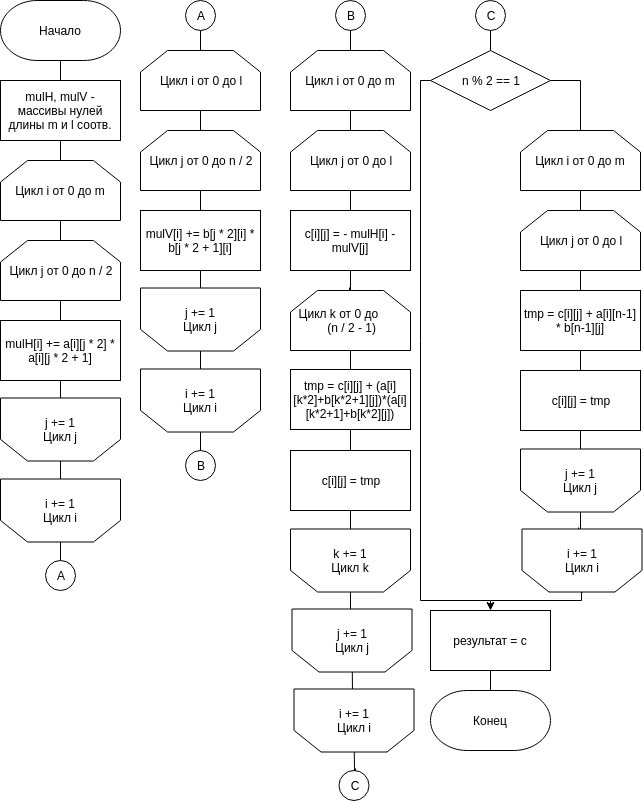
\includegraphics[height=20cm]{vinograd.png}}
\caption{Схема алгоритма Винограда}
\label{fig:image}
\end{figure}

\begin{figure}
\center{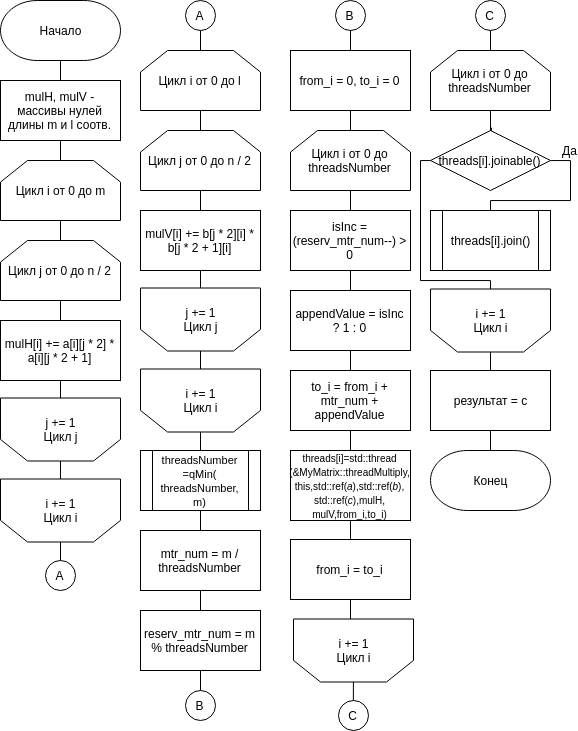
\includegraphics[height=20cm]{vinogradParallel.png}}
\caption{Схема параллельного алгоритма Винограда}
\label{fig:image}
\end{figure}

\begin{figure}
\center{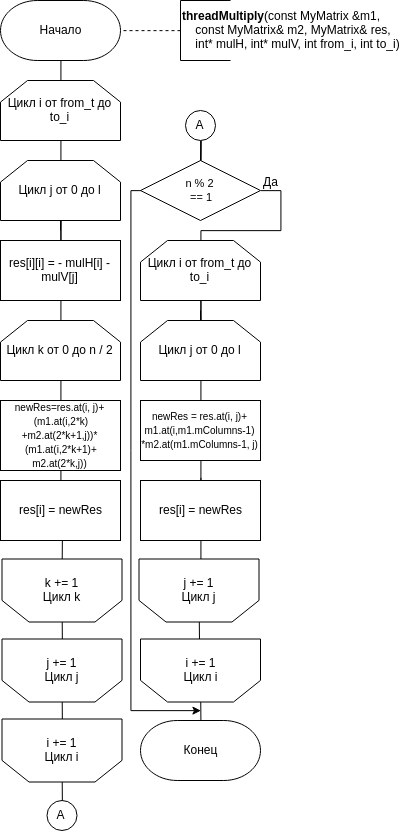
\includegraphics[height=20cm]{threadMult.png}}
\caption{Схема метода threadMultiply, передаваемого каждому потоку}
\label{fig:image}
\end{figure}

\chapter*{Технологическая часть}
\addcontentsline{toc}{chapter}{Технологическая часть}

\section*{Выбор языка программирования}
\addcontentsline{toc}{section}{Выбор языка программирования}

В качестве языка программирования для реализации программы был выбран язык C++ и фреймворк Qt, потому что:
\begin{itemize}
	\item язык C++ имеет высокую вычислительную производительность;
	\item язык C++ поддерживает различные стили программирования;
	\item в Qt существует удобный инструмент для тестирования - QtTest - который позволяет собирать тесты в группы, собирать результаты выполнения тестов, а также уменьшить дублирование кода при схожих объектах тестирования.
\end{itemize}

Для замеров времени использовался методы restart() и elapsed() класса QTime. Метод elapsed() возвращает количество миллисекунд, прошедших с момента последнего вызова start() или restart(). Для получения более достоверных результатов оптимизации компилятора были отключены (-O0).

\section*{Сведения о модулях программы}
\addcontentsline{toc}{section}{Сведения о модулях программы}

Программа состоит из следующих файлов:
\begin{itemize}
	\item mymatrix.h, mymatrix.cpp - заголовочный файл и файл, в котором расположена реализация алгоритмов умножения матриц;
	\item main.cpp - главный файл программы, в котором расположена реализация меню;
	\item testmymatrix.h, testmymatrix.cpp - файл и заголовочный файл, в котором расположена реализация тестов.
\end{itemize}


\section*{Листинги кода алгоритмов}
\addcontentsline{toc}{section}{Листинги кода алгоритмов}

Код алгоритма Винограда представлен в листинге 1. Код параллельного алгоритма Винограда представлен в листинге 2. Код метода, который передается каждому рабочему потоку, представлен в листинге 3.

\begin{lstlisting}[label=some-code,caption=Алгоритм Винограда]
MyMatrix MyMatrix::multiplyVinograd(const MyMatrix &m)
{
    if (mColumns != m.mRows)
        throw std::logic_error("Attempt to multiply matrices of different dimensions.");

    MyMatrix result(mRows, m.mColumns, 0);

    if (result.mColumns == 0 && result.mRows == 0)
        return result;

    int* mulH = new int[result.mRows]{0};
    int* mulV = new int[result.mColumns]{0};

    for (int i = 0; i < result.mRows; ++i)
        for (int j = 0; j < m.mRows / 2; ++j)
            mulH[i] += this->at(i, j * 2) * this->at(i, j * 2 + 1);

    for (int i = 0; i < result.mColumns; ++i)
        for (int j = 0; j < m.mRows / 2; ++j)
            mulV[i] += m.at(2 * j, i) * m.at(j * 2 + 1, i);

    for (int i = 0; i < result.mRows; ++i)
        for (int j = 0; j < result.mColumns; ++j)
        {
            result.set(i, j, - mulH[i] - mulV[j]);
            for (int k = 0; k < m.mRows / 2; ++k)
            {
                int newRes = result.at(i, j) +
                             (this->at(i, 2 * k) + m.at(2 * k + 1, j)) *
                             (this->at(i, 2 * k + 1) + m.at(2 * k, j));
                result.set(i, j, newRes);
            }
        }

    if (mColumns % 2)
    {
        for (int i = 0; i < mRows; ++i)
            for (int j = 0; j < m.mColumns; ++j)
            {
                int newRes = result.at(i, j) +
                             this->at(i, mColumns - 1) *
                             m.at(mColumns - 1, j);
                result.set(i, j, newRes);
            }
    }
    delete [] mulH;
    delete [] mulV;
    return result;
}
\end{lstlisting}

\begin{lstlisting}[label=some-code,caption=Параллельный алгорим Винограда]
MyMatrix MyMatrix::multiplyVinograd_multithread(const MyMatrix &m, int threadsNumber)
{
    if (threadsNumber < 0)
        throw std::logic_error("Threads number is under zero.");

    if (mColumns != m.mRows)
        throw std::logic_error("Attempt to multiply matrices of different dimensions.");

    MyMatrix result(mRows, m.mColumns, 0);

    if (result.mColumns == 0 && result.mRows == 0)
        return result;

    int* mulH = new int[result.mRows]{0};
    int* mulV = new int[result.mColumns]{0};

    for (int i = 0; i < result.mRows; ++i)
        for (int j = 0; j < m.mRows / 2; ++j)
            mulH[i] += this->at(i, j * 2) * this->at(i, j * 2 + 1);

    for (int i = 0; i < result.mColumns; ++i)
        for (int j = 0; j < m.mRows / 2; ++j)
            mulV[i] += m.at(2 * j, i) * m.at(j * 2 + 1, i);

    std::vector<std::thread> threads;
    threadsNumber = qMin(threadsNumber, this->mRows);
    int mtr_num = this->mRows / threadsNumber;
    int reserv_mtr_num = this->mRows % threadsNumber;
    int from_i = 0, to_i;
    for (int i = 0; i < threadsNumber; ++i)
    {
        bool isInc = (reserv_mtr_num--) > 0;
        int appendValue = isInc ? 1 : 0;
        to_i = from_i + mtr_num + appendValue;
        threads.push_back(std::thread(&MyMatrix::threadMultiply, this, std::ref(*this), std::ref(m), std::ref(result), mulH, mulV, from_i, to_i));
        from_i = to_i;
    }

    for (int i = 0; i <  threadsNumber; ++i)
    {
        if (threads.at(i).joinable())
            threads.at(i).join();
    }

    delete [] mulH;
    delete [] mulV;

    return result;
}
\end{lstlisting}


\begin{lstlisting}[label=some-code,caption=\text{Метод threadMultiply, передаваемый каждому потоку}]
void MyMatrix::threadMultiply(const MyMatrix &m1, const MyMatrix& m2, MyMatrix& res, int* mulH, int* mulV, int from_i, int to_i)
{
    for (int i = from_i; i < to_i; ++i)
        for (int j = 0; j < m2.mColumns; ++j)
        {
            res.set(i, j, - mulH[i] - mulV[j]);
            for (int k = 0; k < m2.mRows / 2; ++k)
            {
                int newRes = res.at(i, j) +
                             (m1.at(i, 2 * k) + m2.at(2 * k + 1, j)) *
                             (m1.at(i, 2 * k + 1) + m2.at(2 * k, j));
                res.set(i, j, newRes);
            }
        }

    if (m1.mColumns % 2 == 1)
    {
        for (int i = from_i; i < to_i; ++i)
            for (int j = 0; j < m2.mColumns; ++j)
            {
                int newRes = res.at(i, j) +
                             m1.at(i, m1.mColumns - 1) *
                             m2.at(m1.mColumns - 1, j);
                res.set(i, j, newRes);
            }
    }
}
\end{lstlisting}


\section*{Тесты}
\addcontentsline{toc}{section}{Тесты}

Тестирование проводилось с помощью модуля QtTest. Для этого был написан класс TestMyMatrix. Сначала каждый алгоритм умножения матриц тестировался по отдельности на заранее заготовленном наборе тестовых данных.
После этого генерировались пары случайных квадратных матриц целых чисел в диапазоне от -50 до 50 размером от 0 до 200 с шагом 5 (для каждой размерности матрицы генерировалось 10 случайных матриц). Проводилоь умножение этих пар матриц с помощью алгорима Винограда и параллельного алгорима Винограда и сравнивались результаты работы этих двух алгоритмов. Затем генерировались пары случайных прямоугольных матриц целых чисел в диапазоне от -50 до 50 размером от 0 до 200 с шагом 5 (для каждой размерности матрицы генерировалось 10 случайных матриц). Проводилась умножение этих пар матриц с алгорима Винограда и параллельного алгорима Винограда и сравнивались результаты работы этих двух алгоритмов.

Все написанные тесты были пройдены.

Использованный набор тестовых данных приведен в таблице 1.

\begin{table}[h!]
	\caption{Набор тестовых данных}
	%\begin{center}
		\begin{tabular}{|c | c | c |}
	 	\hline
		Матрица 1 & Матрица 2 & Ожидаемый результат \\ [0.5ex]
	 	\hline\hline
		[0] & [0] & [0] \\
		\hline
		[0] & [1] & [0] \\
		\hline
		[1] & [1] & [1] \\
		\hline
		[2] & [2] & [4] \\
		\hline
		$\begin{bmatrix}
		1 & 1 \\
		1 & 1 \\
		\end{bmatrix}$ &
		$\begin{bmatrix}
		1 & 1 \\
		1 & 1 \\
		\end{bmatrix}$ &
		$\begin{bmatrix}
		2 & 2 \\
		2 & 2 \\
		\end{bmatrix}$ \\
		\hline
		$\begin{bmatrix}
		2 & 2 \\
		2 & 2 \\
		\end{bmatrix}$ &
		$\begin{bmatrix}
		2 & 2 \\
		2 & 2 \\
		\end{bmatrix}$ &
		$\begin{bmatrix}
		8 & 8 \\
		8 & 8 \\
		\end{bmatrix}$ \\
		\hline

		$\begin{bmatrix}
		0 & 0 \\
		0 & 0 \\
		\end{bmatrix}$ &
		$\begin{bmatrix}
		0 & 0 \\
		0 & 0 \\
		\end{bmatrix}$ &
		$\begin{bmatrix}
		0 & 0 \\
		0 & 0 \\
		\end{bmatrix}$ \\
		\hline

		$\begin{bmatrix}
		0 & 0 \\
		0 & 0 \\
		\end{bmatrix}$ &
		$\begin{bmatrix}
		1 & 1 \\
		1 & 1 \\
		\end{bmatrix}$ &
		$\begin{bmatrix}
		0 & 0 \\
		0 & 0 \\
		\end{bmatrix}$ \\
		\hline

		$\begin{bmatrix}
		1 & 2 \\
		3 & 4 \\
		\end{bmatrix}$ &
		$\begin{bmatrix}
		1 & 1 \\
		1 & 1 \\
		\end{bmatrix}$ &
		$\begin{bmatrix}
		3 & 3 \\
		7 & 7 \\
		\end{bmatrix}$ \\
		\hline

		$\begin{bmatrix}
		1 & 1 \\
		1 & 1 \\
		\end{bmatrix}$ &
		$\begin{bmatrix}
		1 & 2 \\
		3 & 4 \\
		\end{bmatrix}$ &
		$\begin{bmatrix}
		4 & 6 \\
		4 & 6 \\
		\end{bmatrix}$ \\
		\hline

		$\begin{bmatrix}
		1 & 2 \\
		3 & 4 \\
		\end{bmatrix}$ &
		$\begin{bmatrix}
		1 & 2 \\
		3 & 4 \\
		\end{bmatrix}$ &
		$\begin{bmatrix}
		7 & 10 \\
		15 & 22 \\
		\end{bmatrix}$ \\
		\hline

		$\begin{bmatrix}
		1 \\
		1 \\
		\end{bmatrix}$ &
		$\begin{bmatrix}
		1 & 1 \\
		\end{bmatrix}$ &
		$\begin{bmatrix}
		1 & 1 \\
		1 & 1 \\
		\end{bmatrix}$ \\
		\hline

		$\begin{bmatrix}
		1 & 1\\
		\end{bmatrix}$ &
		$\begin{bmatrix}
		1 \\
		1 \\
		\end{bmatrix}$ &
		$\begin{bmatrix}
		1 & 1 \\
		1 & 1 \\
		\end{bmatrix}$ \\
		\hline

		$\begin{bmatrix}
		1 & 2 \\
		3 & 4 \\
		5 & 6 \\
		\end{bmatrix}$ &
		$\begin{bmatrix}
		6 & 5 & 4 \\
		3 & 2 & 1\\
		\end{bmatrix}$ &
		$\begin{bmatrix}
		12 & 9 & 6 \\
		30 & 23 & 16 \\
		48 & 37 & 26 \\
		\end{bmatrix}$ \\
		\hline

		$\begin{bmatrix}
		1 & 4 & 8 \\
		16 & 32 & 64 \\
		\end{bmatrix}$ &
		$\begin{bmatrix}
		1 & 3 \\
		9 & 27 \\
		81 & 243 \\
		\end{bmatrix}$ &
		$\begin{bmatrix}
		685 & 2055 \\
		5488 & 16464 \\
		\end{bmatrix}$ \\
		\hline

		$\begin{bmatrix}
		1 & 4 & 1 \\
		5 & 9 & 2 \\
		6 & 5 & 3 \\
		5 & 8 & 9 \\
		\end{bmatrix}$ &
		$\begin{bmatrix}
		7 & 9 & 3 & 2 \\
		3 & 8 & 4 & 6 \\
		2 & 6 & 4 & 3 \\
		\end{bmatrix}$ &
		$\begin{bmatrix}
		21 & 47 & 23 & 29 \\
		66 & 129 & 59 & 70 \\
		63 & 112 & 50 & 51 \\
		77 & 163 & 83 & 85 \\
		\end{bmatrix}$ \\
		\hline

		\end{tabular}
	%\end{center}
\end{table}

\chapter*{Исследовательская часть}
\addcontentsline{toc}{chapter}{Исследовательская часть}

\section*{Постановка эксперимента}
\addcontentsline{toc}{section}{Постановка эксперимента}

В рамках данной работы были проведены следующие эксперименты.

\begin{enumerate}
	\item Замеры времени работы алгорима Винограда для квадратных матриц размерностей от 100 x 100 до 1000 x 1000 с шагом 100.
	\item Замеры времени работы параллельного алгорима Винограда для квадратных матриц размерностей от 100 x 100 до 1000 x 1000 с шагом 100.
	\item Замеры времени работы алгорима Винограда для квадратных матриц размерностей от 101 x 101 до 1001 x 1001 с шагом 100.
	\item Замеры времени работы параллельного алгорима Винограда для квадратных матриц размерностей от 101 x 101 до 1001 x 1001 с шагом 100.
\end{enumerate}

В рамках каждого эксперимента для матриц каждой размерности проводилось по 10 замеров, и вычислялось среднее время работы конкретного алгоритма на матрицах данной размерности.

Измерения проводились на компьютере HP Pavilion Notebook на базе Intel Core i5-7200U, 2.50 Гц с 6 Гб оперативной памяти и с 4 логическими ядрами под управлением операционной системы Linux Mint.

\section*{Сравнительный анализ на материале экспериментальных данных}
\addcontentsline{toc}{section}{Сравнительный анализ на материале экспериментальных данных}

В таблице 1 представлены результаты замеров времени работы алгоритма Винограда (0, мс) и параллельного алгорима Винограда на одном потоке (1, мс), на двух потоках (2, мс) и т.д. на квадратных матрицах четного размера (размерность матрицы указана в столбце "Р-ть") в миллисекундах.
В таблице 2 представлены результаты замеров времени работы алгоритма Винограда (0, мс) и параллельного алгорима Винограда на одном потоке (1, мс), на двух потоках (2, мс) и т.д. на квадратных матрицах нечетного размера (размерность матрицы указана в столбце "Р-ть") в миллисекундах.

\begin{table}
	\caption{Результаты замеров времени для матриц четного размера}
	%\begin{center}
	\tabcolsep=0.11cm
		\begin{tabular}{|c | c | c | c | c | c | c | c | c | c | c | c | c | c | c | c | c | c | c | c | c |}
	 	\hline
		Р-ть & 0, мс & 1, мс & 2, мс & 4, мс & 8, мс & 16, мс \\ [0.5ex]
	 	\hline\hline
		100 & 16 & 20 & 9 & 8 & 7 & 8 \\ \hline
		200 & 133 & 133 & 66 & 62 & 63 & 61 \\ \hline
		300 & 452 & 457 & 228 & 210 & 216 & 212 \\ \hline
		400 & 1077 & 1080 & 541 & 501 & 510 & 506 \\ \hline
		500 & 2147 & 2155 & 1073 & 998 & 995 & 986 \\ \hline
		600 & 3728 & 3861 & 2019 & 1710 & 1716 & 1714 \\ \hline
		700 & 6063 & 6115 & 3042 & 2855 & 2871 & 2745 \\ \hline
		800 & 9288 & 9408 & 4625 & 4191 & 4210 & 4207 \\ \hline
		900 & 13724 & 13870 & 7087 & 6330 & 6320 & 6341 \\ \hline
		1000 & 19275 & 19374 & 10407 & 9089 & 9181 & 9238 \\ \hline
	\end{tabular}
	%\end{center}
\end{table}

\begin{table}
	\caption{Результаты замеров времени для матриц нечетного размера}
	%\begin{center}
	\tabcolsep=0.11cm
		\begin{tabular}{|c | c | c | c | c | c | c | c | c | c | c | c | c | c | c | c | c | c | c | c | c |}
	 	\hline
		Р-ть & 0, мс & 1, мс & 2, мс & 4, мс & 8, мс & 16, мс \\ [0.5ex]
	 	\hline\hline
		101 & 17 & 27 & 9 & 9 & 8 & 8 \\ \hline
		201 & 135 & 136 & 69 & 62 & 64 & 62 \\ \hline
		301 & 458 & 459 & 230 & 215 & 215 & 214 \\ \hline
		401 & 1096 & 1116 & 561 & 509 & 519 & 510 \\ \hline
		501 & 2147 & 2167 & 1078 & 994 & 1006 & 996 \\ \hline
		601 & 3775 & 3786 & 1903 & 1804 & 1746 & 1742 \\ \hline
		701 & 6181 & 6224 & 3074 & 2788 & 2828 & 2882 \\ \hline
		801 & 9458 & 9520 & 4870 & 4231 & 4350 & 4213 \\ \hline
		901 & 14023 & 14089 & 7164 & 6304 & 6335 & 6330 \\ \hline
		1001 & 19596 & 19680 & 10036 & 9192 & 9389 & 9386 \\ \hline
	\end{tabular}
	%\end{center}
\end{table}

\newpage

На рисунке 4 представлены результаты замеров времени работы алгоритма Винограда (noThreadEven) и параллельного алгорима Винограда на одном потоке (thread1Even), на двух потоках (thread2Even), на четырех потоках (thread4Even), на восьми потоках (thread8Even) и на шестнадцати потоках (thread16Even) на квадратных матрицах четного размера.

На рисунке 5 представлены результаты замеров времени работы алгоритма Винограда (noThreadEven) и параллельного алгорима Винограда на одном потоке (thread1Even), на двух потоках (thread2Even), на четырех потоках (thread4Even), на восьми потоках (thread8Even) и на шестнадцати потоках (thread16Even) на квадратных матрицах нечетного размера.


\begin{figure}[!h]
	\begin{minipage}[h]{\linewidth}
	\center{
	\begin{tikzpicture}[scale=2]
	\begin{axis}[
		small,
		%transpose legend,
		legend columns=2,
		legend style = {at={(0.5, -0.3)}, anchor=north},
	    	axis lines = left,
	    	xlabel = {размерность},
	    	ylabel = {время, с},
		ymajorgrids=true
	]
	\scriptsize
	\addplot[color=blue, mark=square] table[x index=0, y index=1] {noThreadEven.dat};
	\addplot[color=green, mark=square] table[x index=0, y index=1] {thread1Even.dat};
	\addplot[color=black, mark=square] table[x index=0, y index=1] {thread2Even.dat};
	\addplot[color=brown, mark=square] table[x index=0, y index=1] {thread4Even.dat};
	\addplot[color=yellow, mark=square] table[x index=0, y index=1] {thread8Even.dat};
	\addplot[color=violet, mark=square] table[x index=0, y index=1] {thread16Even.dat};

	\scriptsize
	\addlegendentry{noThreadEven}
	\addlegendentry{thread1Even}
	\addlegendentry{thread2Even}
	\addlegendentry{thread4Even}
	\addlegendentry{thread8Even}
	\addlegendentry{thread16Even}
	\end{axis}
\end{tikzpicture}
\caption{Результаты замеров времени для матриц четного размера}}
\end{minipage}
\end{figure}

\begin{figure}[!h]
	\begin{minipage}[h]{\linewidth}
	\center{
	\begin{tikzpicture}[scale=2]
	\begin{axis}[
		small,
		%transpose legend,
		legend columns=2,
		legend style = {at={(0.5, -0.3)}, anchor=north},
	    	axis lines = left,
	    	xlabel = {размерность},
	    	ylabel = {время, с},
		ymajorgrids=true
	]
	\scriptsize
	\addplot[color=blue, mark=square] table[x index=0, y index=1] {noThreadOdd.dat};
	\addplot[color=green, mark=square] table[x index=0, y index=1] {thread1Odd.dat};
	\addplot[color=black, mark=square] table[x index=0, y index=1] {thread2Odd.dat};
	\addplot[color=brown, mark=square] table[x index=0, y index=1] {thread4Odd.dat};
	\addplot[color=yellow, mark=square] table[x index=0, y index=1] {thread8Odd.dat};
	\addplot[color=violet, mark=square] table[x index=0, y index=1] {thread16Odd.dat};

	\scriptsize
	\addlegendentry{noThreadOdd}
	\addlegendentry{thread1Odd}
	\addlegendentry{thread2Odd}
	\addlegendentry{thread4Odd}
	\addlegendentry{thread8Odd}
	\addlegendentry{thread16Odd}
	\end{axis}
\end{tikzpicture}
\caption{Результаты замеров времени для матриц нечетного размера}}
\end{minipage}
\end{figure}

\newpage

\section*{Выводы}
\addcontentsline{toc}{section}{Выводы}

В результате проведенных экспериментов было установлено, что:

\begin{enumerate}
	\item параллельная реализация алгоритма Винограда с одним рабочим потоком незначительно уступает по времени последовательной реализации алгорима Винограда (из-за небольших затрат времени на создание рабочего потока);
	\item максимальная производительность достигается при 4-х рабочих потоках, что соответствует количеству логических ядер компьютера, на котором проводились эксперименты;
	\item при количестве потоков больше 4-х наблюдается незначительное падение производительности из-за затрат времени на создание рабочих потоков;
	\item параллельный алгоритм при количестве рабочих потоков от 2-х до 16-ти работает быстрее, чем последовательный алгоритм.
\end{enumerate}


\chapter*{Заключение}
\addcontentsline{toc}{chapter}{Заключение}

В ходе данной лабораторной работы были реализованы последовательный и параллельный алгоритмы Винограда.

Было выполнено сравнение зависимости скорости работы данных алгоритмов от размерности матрицы и количества рабочих потоков.

\end{document}
